\documentclass[11pt,a4paper]{report}
\usepackage[utf8]{inputenc}
\usepackage[russian]{babel}
\usepackage[OT1]{fontenc}
\usepackage{amsmath}
\usepackage{amsfonts}
\usepackage{amssymb}
\usepackage{graphicx}
\author{Александр Лаптев, Владислав Борисов}
\title{Документация по проекту Solar System}
\begin{document}

\begin{titlepage}
 \begin{center}
    \large
    МИНИСТЕРСТВО ОБРАЗОВАНИЯ И НАУКИ\\ РОССИЙСКОЙ ФЕДЕРАЦИИ
     
    \textit{ФГБОУ ВО Российской Федерации}
    \vspace{0.5cm}
 
    АЛТАЙСКИЙ ГОСУДАРСТВЕННЫЙ УНИВЕРСИТЕТ
    
    \vspace{0.25cm}
     
    \textit{Институт цифровых технологий, электроники и физики}
    
    \vfill 
    Информатика и вычислительная техника
    \vfill
    \textsc{Групповая работа}\\[5mm]
     
    {\LARGE «Разработка графической программы с использованием библиотеки Tkinter, моделирующую солнечную систему»}
  \bigskip
     
     группа 595, 2 курс
\end{center}
\vfill
 
\newlength{\ML}
\settowidth{\ML}{«\underline{\hspace{0.6cm}}» \underline{\hspace{1cm}}}
\hfill\begin{minipage}{0.5\textwidth}
  Руководитель курса\\
  \underline{\hspace{\ML}} И.\,А.~Шмаков\\
  «\underline{\hspace{0.5cm}}» \underline{\hspace{1cm}} 2020 г.
\end{minipage}%
\bigskip
 
\hfill\begin{minipage}{0.5\textwidth}
  Студенческая группа:\\
  \underline{\hspace{\ML}} В.\,В.~Борисов \\- кодер\\
  \underline{\hspace{\ML}} А.\,В.~Лаптев  \\- тестировщик / руководитель проекта\\
\end{minipage}%
\vfill
 
\begin{center}
  Барнаул, 2020 г.
\end{center}
\end{titlepage}

\tableofcontents
\newpage
\section{Теория}
\subsection{Python}

Python – высокоуровневый язык программирования общего назначения, ориентированный на повышение производительности разработчика и читаемости кода. Синтаксис ядра Python минималистичен. Такая псевдо-кодовая природа Python является одной из его самых сильных сторон. Она позволяет вам сосредоточиться на решении задачи, а не на самом языке. В то же время стандартная библиотека включает большой набор полезных функций.

Python поддерживает структурное, обобщенное, объектно-ориентированное, функциональное и аспектно-ориентированное программирование. Основные архитектурные черты — динамическая типизация, автоматическое управление памятью, полная интроспекция, механизм обработки исключений, поддержка многопоточных вычислений, высокоуровневые структуры данных. Поддерживается разбиение программ на модули, которые, в свою очередь, могут объединяться в пакеты.

На Python легко начать программировать. Python обладает исключительно простым синтаксисом, как уже говорилось выше.

Python – это пример свободного и открытого программного обеспечения –FLOSS (Free/Libré and Open Source Software). Вы имеете право свободно распространять копии этого программного обеспечения, читать его исходные тексты, вносить изменения, а также использовать его части в своих программах. В основе свободного ПО лежит идея сообщества, которое делится своими знаниями. Это одна из причин, по которым Python так хорош: он был создан и постоянно улучшается сообществом, которое просто хочет сделать его лучше.

При написании программы на Python вам никогда не придётся отвлекаться на такие низкоуровневые детали, как управление памятью, используемой вашей программой, и т.п.

Благодаря своей открытой природе, Python был портирован на много платформ (т.е. изменён таким образом, чтобы работать на них). Все ваши программы смогут запускаться на любой из этих платформ без каких-либо изменений, если только вы избегали использования системно-зависимых функций.

Программа, написанная на компилируемом языке программирования, как например, C++, преобразуется из исходного языка в язык, понятный компьютеру (бинарный код) при помощи компилятора с применением разнообразных флагов и параметров. Когда вы запускаете такую программу, компоновщик/загрузчик копирует программу с диска в оперативную память и запускает её.  Python же, напротив, не требует компиляции в бинарный код. Программа просто выполняется из исходного текста. Python сам преобразует этот исходный текст в некоторую промежуточную форму, называемую байткодом, а затем переводит его на машинный язык и запускает. Всё это заметно облегчает использование Python, поскольку нет необходимости заботиться о компиляции программы, подключении и загрузке нужных библиотек и т. д. Вместе с тем, это делает программы на Python намного более переносимыми, так как достаточно их просто скопировать на другой компьютер, и они работают.

Python поддерживает как процедурно-ориентированное, так и объектно-ориентированное программирование. В процедурно-ориентированных языках программы строятся на основе процедур или функций, которые представляют собой просто-напросто многократно используемые фрагменты программы. В объектно-ориентированных языках программирования программы строятся на основе объектов, объединяющих в себе данные и функционал. Python предоставляет простые, но мощные средства для ООП, особенно в сравнении с такими большими языками программирования, как C++ или Java.

Если вам нужно, чтобы некоторая критическая часть программы работала очень быстро или вы вынуждены скрыть часть алгоритма, вы можете написать эту часть программы на C или C++, а затем вызывать её из программы на Python.

Python можно встраивать в программы на C/C++, чтобы предоставлять возможности написания сценариев их пользователям.

Стандартная библиотека Python просто огромна. Она может помочь в решении разнообразных задач, связанных с использованием регулярных выражений, генерированием документации, проверкой блоков кода, распараллеливанием процессов, базами данных, веб-браузерами, CGI, FTP, электронной почтой, XML, XML-RPC, HTML, WAV файлами, криптографией, GUI (графическим интерфейсом пользователя) и другими системно-зависимыми вещами. Помните, что всё это доступно абсолютно везде, где установлен Python. В этом заключается философия Python «Всё включено».

\subsection{Tkinter}
Tkinter – это кроссплатформенная библиотека для разработки графического интерфейса на языке Python (начиная с Python 3.0 переименована в tkinter). кросс-платформенная событийно-ориентированная графическая библиотека на основе средств Tk (широко распространённая в мире GNU/Linux и других UNIX‐подобных систем, портирована также и на Windows и macOS), написанная Стином Лумхольтом и Гвидо ван Россумом. Tkinter расшифровывается как Tk interface, и является интерфейсом к Tcl/Tk.

Tkinter входит в стандартный дистрибутив Python.

Визуальные элементы отображаются через собственные элементы текущей операционной системы, поэтому приложения, созданные с помощью Tkinter, выглядят так, как будто они принадлежат той платформе, на которой они работают.

У Tkinter есть свои недостатки. Один из них заключается в том, что графические интерфейсы, созданные с использованием Tkinter, выглядят устаревшими. Для более современного интерфейса есть PyQt5 который сильнее подходит для данных целей.

Тем не менее, в плане использования, Tkinter является более простым по сравнению с другими библиотеками. Это хороший выбор для создания GUI приложений в Python если большую роль играет функциональность и кроссплатформенная скорость.

\subsection{Выбранный язык программирования}
Основным языком программирования (далее ЯП) стал Python. Главными факторами при выборе языка стали:
\begin{enumerate}
    \item Высокая скорость написания программы
    \item Большое количество документации по языку и дополнительным пакетам
    \item Богатая библиотека пакетов, таких как \textit{Tkinter} 
\end{enumerate} 
\section{Постановка задачи}
Разработать программу, которая  будет отображать схематичную модель солнечной системы, с указанием информации о каждой  планете, при нажатии на соответствующую планету. 

\section{Цель проекта}
Разработать программу, отображающую модель и поведение солнечной системы. Интерфейс программы должен быть выполнен с использованием библиотеки \textit{Tkinter}. Программа должна быть написана с использованием парадигмы ООП.

\section{Описание классов}
Перед описанием классов хотелось рассказать про создание нескольких переменных и кнопки с помощью которой происходит увеличение скорости планет.
Пришлось отдельно (вне классов) создать две глобальные переменные angle и izmen,которые равны нулю.Первая переменная используется для создания движения планет по окружности (опис. ниже),второя для изменения этой скорости.Они сделаны глобальными,потому что используются как внутри, так и вне классов.
Затем создается отдельная функция speed которая содержит глобальную переменную izmen(коэффициэнт ускорения планеты).Изначально он равен нулю,но при вызове самой функции он увеличивается на 0.001,если коэффициэнт становится больше чем 0.004,то он обнуляется.Таким образом после того как мы свяжем созданную кнопку с данной функцией мы сможем изменять параметр ускорения планеты 4 раза после чего скорость планеты вернется к изначальной.
\begin{verbatim}
    angle=0
    izmen=0
    def speed():
       global izmen   
       izmen+=+0.001
       if izmen==0.004:
           izmen=0
    #создаем кнопку и привязываем функцию   
    button = tk.Button(root,
        text="скорость!",
        width=7,
        height=2,
        bg="black",
        fg="white",
        command=speed)
    button.place(x=1030,y=300)
\end{verbatim}
\subsection{Класс Planet}
Класс Planet  - содержит методы и функции для графического представления планет. В нём описаны методы для отрисовки планет на слое, перемещение планет, относительно Солнца -левый нижний край экрана.
В методе init у нас будет происходить отрисовка планеты,а также "добавление планеты очков  жизни"(с помощью очков проиходит движение планет).
Далее для каждой планеты есть своя функция которая содержит следующие переменные: х,y-координаты планеты в прострастве,r-радиус планеты,хn,yn-координаты точки вокруг которой будет вращаться планета(она у всех одинаковая),собственный цвет,v- сдвиг от точки спавна по х и у,собственное имя,которое мы будем отображать на планете,а также связывание с окном описания планеты, которое вызывается при нажатии на планету.Внимание !!!. Функция sun не содержит переменныех xn,yn,v, т.к. солнце не движется.

Данная функция задается следующим кодом:
\begin{verbatim}
class planet():
    def __init__(self):
        self.id = cosmos.create_oval(0,0,0,0)
        self.live=1
        
    def solnce(self):
        x=self.x=0
        y=self.y=708
        r=self.r=125
        color=self.color="yellow"
        cosmos.coords(self.id, x-r, y-r, x+r, y+r)
        cosmos.create_text(self.x+24,self.y-10,text='солнце')
        cosmos.itemconfig(self.id, fill=color)
        cosmos.tag_bind(self.id, '<Button-1>', UI.Sun)
      
        
    def mercury(self):
        x=self.x=0    #координата по х
        y=self.y=558 # координата по у
        r=self.r=26  # радиус планеты
        self.xn=0 #  !!!точка вокруг которой вращаются планеты!!!
        self.yn=708 #!!!точка вокруг которой вращаются планеты!!!
        self.rv=165 #!!! собственный радиус вращения!!!
        self.v=+1.0 # !!! координата сдвига спавна 
        color=self.color="white"
        cosmos.coords(self.id, x-r, y-r, x+r, y+r)
        cosmos.itemconfig(self.id, fill=color) 
        self.name="меркурий"
        self.txt=cosmos.create_text(self.x,self.y,text=self.name) # создаем текст на 
        планете
        cosmos.tag_bind(self.id, '<Button-1>', UI.Mercury) # связываем окно с 
        планетой по нажатию  лкм по планете
\end{verbatim}
Далее используется функция движения планеты.Она содержит две глобальные переменные angle(угол), и izmen(коэффициэнт ускорения),а которых мы говорили выше,в этой функции angle будет изменяться на 0.0013+izmen каждый раз.После того как угол становится больше 360, то angle обнуляется.Переменные х и у составляют уравнение окружности,благодаря ним проиходит смещение планеты.Также в функции происходит удаление старого текста с названием планеты, который расположен по старым координатам, и отрисовка нового.

\begin{verbatim}
 def move(self):
    global angle,izmen       # угол поворота и изменение скорости вращения 
    angle+=0.0013+izmen      # угол изменяется на число каждый раз
    if angle>=360:           #если =360 то зануляем
            angle=0
    self.x =self.xn+ self.rv* math.sin(angle-self.v)    # изменение координат планет 
    в космосе 
    self.y =self.yn+ self.rv* math.cos(angle-self.v)    # изменение координат планет 
    в космосе
    cosmos.delete(self.txt)                             #удаляем старое название 
    планеты т.к нужно отрисовать в новом месте ( собст имя создали в функ )
    self.txt=cosmos.create_text(self.x,self.y,text=self.name) # рис новое имя
    self.set_coords()   
\end{verbatim}



\subsection{Класс UI}

Класс UI - один из классов, в программе. Данный класс предназначен для отрисовки окна с краткой информацией о каждой планете.
Класс UI содержит функции, в которых происходит создание окна  - info, добавление заголовка планеты - Lab, добавление изображения планеты - img. 
Для реализации окна, будем использовать метод \textit{Toplevel}, данный способ позволяет создать окно, которое будет всегда находиться поверх основной программы. 
Подобный метод создания окна имеет следующие плюсы:
\begin{enumerate}
    \item Возможность открывать несколько окон, к примеру, для сравнения характеристик планет
    \item Модель Солнечной системы, при желании, можно переместить в свободную область, т.о иметь возможность наблюдать модель Солнечной системы и видеть информацию об интересующей планете
    \item Наличие 2 отдельных окон (основное и окно с информацией), что несколько упрощает разработку кода
\end{enumerate}
Создание окна с информацией:
\begin{verbatim}
#Создаем окно вверхнего уровня
    info = tk.Toplevel(root, bg ='black')
#Задаем заголовок окну. В нашем случае это "Инфа по планетам"
    info.title("Инфа по планетам")
#Устанавливаем размер окна
    info.geometry('800x600')
#Запрещаем пользователю менять размер окна
    info.resizable(False,False)
\end{verbatim}
Далее создаем основной   Label размером с окно, на котором разместим маленький лэйбл для фото и несколько полей для ввода текста в которых будем описывать планету :
\begin{verbatim}
    Lab = Label(info, bg='black', fg='white', font='Arial 25',width=800,height=600)
    # основной лэйбл - все окно
        Lab.pack(fill=BOTH,expand=1)
    Lab.pack()
\end{verbatim}
Теперь в верхней правой части окна info создадим  мини лэйбл  в котором будем хранить картинку 
\begin{verbatim}
    photo = PhotoImage(file="MERK.png")         # сама картинка
        img = Label(Lab,image = photo, bg='black') # вставляем картинку в лэйбл
        img.place(x=0,y=0)                          # местоположений
\end{verbatim}        
Создаем  поля для текcта, в первом будем хранить название планеты, во втором ее характеристики, а в третьем просто интересную информацию
\begin{verbatim}
    text_name=Text(Lab, bg='black', fg='white', borderwidth=0, width=300, height=50, 
    font='Arial 25', wrap='word',
                    state='normal')                 # поле для имени
    text_bok=Text(Lab, bg='black', fg='white', borderwidth=0, width=300, height=200, 
    font='Arial 10', wrap='word',
                    state='normal')                  # поле для характеристик
    text_niz = Text(Lab, bg='black', fg='white', borderwidth=0, width=700, 
    height=200, font='Arial 11', wrap='word',
                    state='normal')           
\end{verbatim}


Вставляем текст в нужные поля  
\begin{verbatim}
    text_name.insert(1.0,'                   МЕРКУРИЙ')
    text_name.place(x=300,y=0)#положение имени
    text_bok.insert(1.0,    '           Характеристики Меркурия\n' 
                                'Меркурий является самой маленькой планетой 
                                Солнечной системы.\n'
                                'Радиус Меркурия составляет всего 2440 километров 
                                (38% радиуса Земли)\n'
                                'Температура на поверхности Меркурия колеблется от 
                                −190°C до +430°C.\n'
                                'Солнечная сторона нагревается гораздо больше, 
                                чем полярные области и\n'
                                'обратная сторона планеты.\n'
                                'Меркурий обладает магнитным полем, напряженность 
                                которого примерно\n' 
                                'в 100 раз меньше земного.\n'
                                'Меркурий вторая по плотности (после Земли) планета 
                                в Солнечной\n'
                                'системе.\n'
                                'Ускорение свободного падения на Меркурии равно 3,7 
                                м/c^2 \n'
                                'Площадь поверхности Меркурия составляет 74 797 000 
                                км^2\n' 
                                'Масса Меркурия равна 3,3010 х 1023 килограмма')
        
        
    text_bok.place(x=300,y=71) # расположение хар-к        
    text_niz.insert(1.0,'\n\n \nВыжженный Солнцем Меркурий лишь немного больше, чем 
    спутник Земли Луна.\n'
                        'Подобно Луне, Меркурий практически лишен атмосферы и не 
                        может сгладить следы воздействия от падения\n' 
                        'метеоритов, поэтому он как и Луна покрыт кратерами.\n'
                        'Дневная сторона Меркурия очень сильно нагревается на 
                        Солнце, а на ночной стороне температура падает \n'
                        'на сотни градусов ниже нуля. В кратерах Меркурия, которые 
                        расположены на полюсах, существует лед.\n'
                        'Меркурий совершает один оборот вокруг Солнца за 88 дней.')
    text_niz.place(x=0,y=300) # расположение инфы  
\end{verbatim}
 
\newpage
Итоговый код вывода информации о планете, на примере Меркурия, будет выглядеть так:
\begin{verbatim}
class UI:
    def __init__(self):
        pass
    def Mercury(event):  # Меркурий
        # Подготовка окна с информацией о планете
        info = Toplevel(root, width=800, height=600) # окно
        info.title("Инфа по планетам")  # название
        info.geometry('800x600')       #размер
        info.resizable(False, False)  # Запрет на изменение размера окна
        
        
        
    
        Lab = Label(info, bg='black', fg='white', font='Arial 25',width=800,
        height=600)  # основной лэйбл - все окно
        Lab.pack(fill=BOTH,expand=1)
        global photo
        photo = PhotoImage(file="MERK.png")         # сама картинка
        img = Label(Lab,image = photo, bg='black') # вставляем картинку
        img.place(x=0,y=0)                          # местоположений
        text_name=Text(Lab, bg='black', fg='white', borderwidth=0, width=300, 
        height=50, font='Arial 25', wrap='word',
                    state='normal')                 # поле для имени
        text_bok=Text(Lab, bg='black', fg='white', borderwidth=0, width=300, 
        height=200, font='Arial 10', wrap='word',
                    state='normal')                  # поле для характеристик
        text_niz = Text(Lab, bg='black', fg='white', borderwidth=0, width=700, 
        height=200, font='Arial 11', wrap='word',
                    state='normal')                 # интересн инфа
    
       
        text_name.insert(1.0,'                   МЕРКУРИЙ')
        text_name.place(x=300,y=0)#положение имени
        text_bok.insert(1.0,    '                                           
        Характеристики Меркурия\n' 
                                'Меркурий является самой маленькой планетой 
                                Солнечной системы.\n'
                                'Радиус Меркурия составляет всего 2440 километров 
                                (38% радиуса Земли)\n'
                                'Температура на поверхности Меркурия колеблется от 
                                −190°C до +430°C.\n'
                                'Солнечная сторона нагревается гораздо больше, чем 
                                полярные области и\n'
                                'обратная сторона планеты.\n'
                                'Меркурий обладает магнитным полем, напряженность 
                                которого примерно\n' 
                                'в 100 раз меньше земного.\n'
                                'Меркурий вторая по плотности (после Земли) планета 
                                в Солнечной\n'
                                'системе.\n'
                                'Ускорение свободного падения на Меркурии равно 3,7
                                м/c^2 \n'
                                'Площадь поверхности Меркурия составляет 74 797 000 
                                км^2\n' 
                                'Масса Меркурия равна 3,3010 х 1023 килограмма')
        
        
        text_bok.place(x=300,y=71) # расположение хар-к        
        text_niz.insert(1.0,'\n\n \nВыжженный Солнцем Меркурий лишь немного больше, 
        чем спутник Земли Луна.\n'
                        'Подобно Луне, Меркурий практически лишен атмосферы и не 
                        может сгладить следы воздействия от падения\n' 
                        'метеоритов, поэтому он как и Луна покрыт кратерами.\n'
                        'Дневная сторона Меркурия очень сильно нагревается на 
                        Солнце, а на ночной стороне температура падает \n'
                        'на сотни градусов ниже нуля. В кратерах Меркурия, которые 
                        расположены на полюсах, существует лед.\n'
                        'Меркурий совершает один оборот вокруг Солнца за 88 дней.')
        text_niz.place(x=0,y=300) # расположение ин инфы
\end{verbatim}

Остальные планеты реализованы точно таким же образом, меняется только изображение, название планеты и текст.
Итоговый вид окна можно посмотреть в Приложение 1 (рис.1).
\subsection{Основной код программы}
После инициализации всех классов начинается создание объектов класса \textit{Planet()} с заданными значениями координат x,y и радиуса.
После этого, происходит отрисовка объектов на слое  \textit{canvas}, с  учетом соответсвующих координат и заданым цветом. 

Далее к объектам привязывается гиперссылка, которая при на нажатии ЛКМ вызывает соответствующую функцию, выводящую информацию о планет и  описанную ранее в классе UI.  





Заключительная часть - вызов функций обновления экрана root.mainloop().












\newpage
\section{Приложение 1}
\scriptsize
\begin{verbatim}
import tkinter as tk
from tkinter import*
import math
import time
root = tk.Tk()
root.geometry('1199x756')
root.resizable(width=False, height=False)
cosmos=Canvas(root, width=1199,height=756)
fon = PhotoImage(file="Back.png")
id_img= cosmos.create_image(0,0,anchor=NW,image=fon)
cosmos.pack(fill=BOTH,expand=1)
angle=0
izmen=0
def speed():
       global izmen  #ускорение 
       izmen+=+0.001 
       if izmen==0.004:
           izmen=0
       
       
       
button = tk.Button(root,
    text="скорость!",
    width=7,
    height=2,
    bg="black",
    fg="white",
    command=speed
)
 
button.place(x=1030,y=300)
class UI:
    def __init__(self):
        pass
    def Mercury(event):  # Меркурий
        # Подготовка окна с информацией о планете
        info = Toplevel(root, width=800, height=600) # окно
        info.title("Инфа по планетам")  # название
        info.geometry('800x600')       #размер
        info.resizable(False, False)  # Запрет на изменение размера окна
        
        
        
    
        Lab = Label(info, bg='black', fg='white', font='Arial 25',width=800,height=600)  # основной лэйбл - все 
        окно
        Lab.pack(fill=BOTH,expand=1)
        global photo
        photo = PhotoImage(file="MERK.png")         # сама картинка
        img = Label(Lab,image = photo, bg='black') # вставляем картинку
        img.place(x=0,y=0)                          # местоположений
        text_name=Text(Lab, bg='black', fg='white', borderwidth=0, width=300, height=50, font='Arial 25', 
        wrap='word',
                    state='normal')                 # поле для имени
        text_bok=Text(Lab, bg='black', fg='white', borderwidth=0, width=300, height=200, font='Arial 10', 
        wrap='word',
                    state='normal')                  # поле для характеристик
        text_niz = Text(Lab, bg='black', fg='white', borderwidth=0, width=700, height=200, font='Arial 11', 
        wrap='word',
                    state='normal')                 # интересн инфа
    
       
        text_name.insert(1.0,'                   МЕРКУРИЙ')
        text_name.place(x=300,y=0)#положение имени
        text_bok.insert(1.0,    '                                           Характеристики Меркурия\n' 
                                'Меркурий является самой маленькой планетой Солнечной системы.\n'
                                'Радиус Меркурия составляет всего 2440 километров (38% радиуса Земли)\n'
                                'Температура на поверхности Меркурия колеблется от −190°C до +430°C.\n'
                                'Солнечная сторона нагревается гораздо больше, чем полярные области и\n'
                                'обратная сторона планеты.\n'
                                'Меркурий обладает магнитным полем, напряженность которого примерно\n' 
                                'в 100 раз меньше земного.\n'
                                'Меркурий вторая по плотности (после Земли) планета в Солнечной\n'
                                'системе.\n'
                                'Ускорение свободного падения на Меркурии равно 3,7 м/c^2 \n'
                                'Площадь поверхности Меркурия составляет 74 797 000 км^2\n' 
                                'Масса Меркурия равна 3,3010 х 1023 килограмма')
        
        
        text_bok.place(x=300,y=71) # расположение хар-к        
        text_niz.insert(1.0,'\n\n \nВыжженный Солнцем Меркурий лишь немного больше, чем спутник Земли Луна.\n'
                        'Подобно Луне, Меркурий практически лишен атмосферы и не может сгладить следы 
                        воздействия от падения\n' 
                        'метеоритов, поэтому он как и Луна покрыт кратерами.\n'
                        'Дневная сторона Меркурия очень сильно нагревается на Солнце, а на ночной стороне 
                        температура падает \n'
                        'на сотни градусов ниже нуля. В кратерах Меркурия, которые расположены на полюсах, 
                        существует лед.\n'
                        'Меркурий совершает один оборот вокруг Солнца за 88 дней.')
        text_niz.place(x=0,y=300) # расположение ин инфы  
                                              
                                            #!!! ОСТАЛЬНЫЕ ПЛАНЕТЫ СДЕЛАНЫ ТОЧНО ТАКЖЕ!!!!
        
    def Venera(event):  
        info = Toplevel(root, width=800, height=600)
        info.title("Инфа по планетам")
        info.geometry('800x600')
        info.resizable(False, False)  
        
    
        
    
        Lab = Label(info, bg='black', fg='white', font='Arial 25',width=800,height=600)  
        Lab.pack(fill=BOTH,expand=1)
        global photo
        photo = PhotoImage(file="ven.png")
        img = Label(Lab,image = photo, bg='black')
        img.place(x=0,y=50)
        text_name=Text(Lab, bg='black', fg='white', borderwidth=0, width=300, height=50, font='Arial 25', 
        wrap='word',
                    state='normal')  
        text_bok=Text(Lab, bg='black', fg='white', borderwidth=0, width=300, height=200, font='Arial 10', 
        wrap='word',
                    state='normal')  
        text_niz = Text(Lab, bg='black', fg='white', borderwidth=0, width=700, height=200, font='Arial 11', 
        wrap='word',
                    state='normal')  
    
       
        text_name.insert(1.0,'                   Венера')
        text_name.place(x=300,y=0)
        text_bok.insert(1.0,    '                                           Характеристики Венеры\n' 
                                  'Температура на поверхности Венеры достигает 477°C.\n'
                                  'Венера шестая по размеру планета в Солнечной системе.\n'
                                  'Радиус Венеры составляет 6052 километра (95% радиуса Земли)\n'
                                  'Площадь поверхности Венеры составляет 460 234 317 км^2 \n'
                                  'Венера вторая по плотности (после Земли) планета в Солнечной системе.\n'
                                  'Ускорение свободного падения на Венере равно 8,87 м/c^2\n'
                                  'Масса Венеры равна 4,87 х 1024 килограмма, что составляет\n'
                                  'Венера обладает самой плотной атмосферой среди всех планет земной группы.')    
        
        text_bok.place(x=300,y=71)        
        text_niz.insert(1.0,'\n\n \nВенера это мир чудовищной жары (еще больше чем на Меркурии) и вулканической 
        активности.\n'
                            'Аналогичная по структуре и размеру Земле, Венера покрыта толстой и токсичной 
                            атмосферой,которая\n'
                            'создает сильный парниковый эффект. Этот выжженной мир достаточно горячий, чтобы 
                            расплавить свинец.\n'
                            'Радарные снимки сквозь могучую атмосферу выявили вулканы и деформированные горы.\n'
                            'Венера вращается в противоположном направлении, от вращения большинства планет.')
        text_niz.place(x=0,y=300)
    def Earth(event):  
        info = Toplevel(root, width=800, height=600)
        info.title("Инфа по планетам")
        info.geometry('800x600')
        info.resizable(False, False)  
        
        
    
        Lab = Label(info, bg='black', fg='white', font='Arial 25',width=800,height=600)  
        Lab.pack(fill=BOTH,expand=1)
        global photo
        photo = PhotoImage(file="zemlya.png")
        img = Label(Lab,image = photo, bg='black')
        img.place(x=0,y=50)
        text_name=Text(Lab, bg='black', fg='white', borderwidth=0, width=300, height=50, font='Arial 25', 
        wrap='word',
                    state='normal')  # Задаем текст  с инфой о планете
        text_bok=Text(Lab, bg='black', fg='white', borderwidth=0, width=300, height=200, font='Arial 10', 
        wrap='word',
                    state='normal')  # Задаем текст  с инфой о планете
        text_niz = Text(Lab, bg='black', fg='white', borderwidth=0, width=700, height=200, font='Arial 11', 
        wrap='word',
                    state='normal')  # Задаем текст  с инфой о планете
    
       
        text_name.insert(1.0,'                   Земля')
        text_name.place(x=300,y=0)
        text_bok.insert(1.0,    '                                           Характеристики Земли\n' 
                                  'Земля – пятая по размеру планета в Солнечной системе.\n'
                                  'Температура на поверхности Земли колеблется в пределах от -89,2 до +56,7°C.\n'
                                  'Экваториальный радиус Земли составляет 6378,1 километра.\n'
                                  'Площадь поверхности Земли составляет 510,072 миллиона км^2.\n'
                                  'Средняя плотность Земли составляет 5,5153 грамм на кубический сантиметр.\n'
                                  'Ускорение свободного падения на Земле равно 9,78 м/с^2.\n'
                                  'Масса Земли равна 5,9726 х 1024 килограмма.')    
        
        text_bok.place(x=300,y=71)        
        text_niz.insert(1.0,'\n\n \nЗемля — планета океан. Наш дом, с его обилием воды и жизни делает его 
        уникальным, в нашей Солнечной\n' 
                        'системе Земля занимает особое место.\n'
                        'Другие планеты, в том числе несколько лун, также имеют залежи льда, атмосферу, времена 
                        года и даже погоду,\n'
                        'но только на Земле все эти компоненты собрались вместе таким образом, что стало 
                        возможным существование \n' 
                        'жизни.')
        text_niz.place(x=0,y=300)
    def Mars(event):  
        info = Toplevel(root, width=800, height=600)
        info.title("Инфа по планетам")
        info.geometry('800x600')
        info.resizable(False, False)  
       
        
        
    
        Lab = Label(info, bg='black', fg='white', font='Arial 25',width=800,height=600)  
        Lab.pack(fill=BOTH,expand=1)
        global photo
        photo = PhotoImage(file="mars.png")
        img = Label(Lab,image = photo, bg='black')
        img.place(x=0,y=0)
        text_name=Text(Lab, bg='black', fg='white', borderwidth=0, width=300, height=50, font='Arial 25', 
        wrap='word',
                    state='normal')  # Задаем текст  с инфой о планете
        text_bok=Text(Lab, bg='black', fg='white', borderwidth=0, width=300, height=200, font='Arial 10', 
        wrap='word',
                    state='normal')  # Задаем текст  с инфой о планете
        text_niz = Text(Lab, bg='black', fg='white', borderwidth=0, width=700, height=200, font='Arial 11', 
        wrap='word',
                    state='normal')  # Задаем текст  с инфой о планете
    
       
        text_name.insert(1.0,'                   Марс')
        text_name.place(x=300,y=0)
        text_bok.insert(1.0,    '                                           Характеристики Марса\n' 
                                  'Марс – седьмая по размеру планета в Солнечной системе.\n'
                                  'Температура на поверхности Марса колеблется в пределах от -153 до +35°C.\n'
                                  'Радиус Марса составляет 3389 километров (53% радиуса Земли).\n'
                                  'Площадь поверхности Марса составляет 144,37 миллиона км^2 \n'
                                 'Средняя плотность Марса составляет 3930 кг/м^3 \n'                              
                                 'Ускорение свободного падения на Марсе равно 3,711 м/c^2 \n'
                                 'Масса Марса равна 6,4171 х 1023 килограмма')
        text_bok.place(x=300,y=71)        
        text_niz.insert(1.0,'\n\n \nХотя детали поверхности Марса трудно увидеть с Земли, наблюдения в телескоп 
        показывают,что на Марсе\n'
                        'существуют сезоны и белые пятна на полюсах. В течение многих десятилетий,люди полагали,
                        что яркие\n'
                        'и темные области на Марсе это пятна растительности и что Марс может быть подходящим 
                        местом для жизни,\n'
                        'и что вода существует в полярных шапках.\n'
                        'Когда космический аппарат Маринер-4, прилетел у Марсу в 1965 году, многие из ученых 
                        были потрясены,\n'
                        'увидев фотографии мрачной планеты покрытой кратерами. Марс оказался мертвой 
                        планетой.\n'
                        'Более поздние миссии, однако, показали, что Марс хранит множество тайн, которые еще 
                        предстоит решить.')
        text_niz.place(x=0,y=300)
    def Yupiter(event): 
        info = Toplevel(root, width=800, height=600)
        info.title("Инфа по планетам")
        info.geometry('800x600')
        info.resizable(False, False)  
        
        
        
    
        Lab = Label(info, bg='black', fg='white', font='Arial 25',width=800,height=600)
        Lab.pack(fill=BOTH,expand=1)
        global photo
        photo = PhotoImage(file="yupi.png")
        img = Label(Lab,image = photo, bg='black')
        img.place(x=0,y=50)
        text_name=Text(Lab, bg='black', fg='white', borderwidth=0, width=300, height=50, font='Arial 25', 
        wrap='word',
                    state='normal')  
        text_bok=Text(Lab, bg='black', fg='white', borderwidth=0, width=300, height=200, font='Arial 10', 
        wrap='word',
                    state='normal')  
        text_niz = Text(Lab, bg='black', fg='white', borderwidth=0, width=700, height=200, font='Arial 11', 
        wrap='word',
                    state='normal')  
    
       
        text_name.insert(1.0,'                   Юпитер')
        text_name.place(x=300,y=0)
        text_bok.insert(1.0,    '                                           Характеристики Юпитера\n' 
                                  'Юпитер – первая по размеру планета в Солнечной системе.\n'
                                  'Верхний уровень непрозрачных облаков Юпитера характеризуется\n'
                                  'давлением в 1 атмосферу\n'
                                  'и температурой -107 °C; на глубине 146 километров – 22 атмосферы, +153 °C.\n'
                                  'Средний радиус Юпитера составляет 69 911 ± 6 километров.\n'
                                  'Площадь поверхности Юпитера составляет 62,1796 миллиарда км^2.\n'
                                  'Средняя плотность Юпитера составляет 1,326 грамм на кубический сантиметр.\n'
                                  'Ускорение свободного падения на Юпитера равно 24,79 м/c^2 \n'
                                  'Масса Юпитера равна 1,8986 х 1027 килограмм')
        text_bok.place(x=300,y=71)        
        text_niz.insert(1.0,'\n\n \nЮпитер — самая массивная планета в нашей Солнечной системе, имеет четыре 
        больших спутника и множество\n'
                        'небольших лун.\n'
                        'Юпитер образует своего рода миниатюрную Солнечную систему. Чтобы превратится в 
                        полноценную звезду,\n'
                        'Юпитеру нужно было стать в 80 раз массивнее.')
        text_niz.place(x=0,y=300)
    def Saturn(event): 
        info = Toplevel(root, width=800, height=600)
        info.title("Инфа по планетам")
        info.geometry('800x600')
        info.resizable(False, False) 
        
        Lab = Label(info, bg='black', fg='white', font='Arial 25',width=800,height=600)  
        Lab.pack(fill=BOTH,expand=1)
        
        global photo
        photo = PhotoImage(file="saturn.png")
        img = Label(Lab,image = photo, bg='black')
        img.place(x=0,y=0)
        text_name=Text(Lab, bg='black', fg='white', borderwidth=0, width=300, height=50, font='Arial 25', 
        wrap='word',
                    state='normal')  
        text_bok=Text(Lab, bg='black', fg='white', borderwidth=0, width=300, height=200, font='Arial 10', 
        wrap='word',
                    state='normal')  
        text_niz = Text(Lab, bg='black', fg='white', borderwidth=0, width=700, height=200, font='Arial 11', 
        wrap='word',
                    state='normal')  
    
       
        text_name.insert(1.0,'                   САТУРН')
        text_name.place(x=300,y=0)
        
        
        
        text_bok.insert(1.0,    '                                           Характеристики Сатурна\n' 
                                'Сатурн – вторая по размеру планета в Солнечной системе.\n'
                                'Средний радиус Сатурна составляет 58 232 ± 6 километров\n'
                                'Площадь поверхности Сатурна составляет 42,72 миллиарда км^2.\n'
                                'Средняя плотность Сатурна составляет 0,687 грамм на кубический сантиметр.\n'
                                'Ускорение свободного падения на Сатурне равно 10,44 м/c^2\n'
                                'Масса Сатурна равна 5,6846 х 1026 кг')
        
        
        text_bok.place(x=300,y=71)        
        
        
        text_niz.insert(1.0,'\n\n \nСатурн — самая дальняя из пяти планет, которые были известны до изобретения 
        телескопа. Подобно Юпитеру,\n'
                         'Сатурн состоит в основном из водорода и гелия. Его объем в 755 раз больше, чем у 
                         Земли. Ветры в его атмосфере\n'
                         'достигают скорости 500 метров в секунду. Эти быстрые ветра в сочетании с теплом, 
                         поднимающимся из недр\n' 
                         'планеты,вызывают появление желтых и золотистых полос, которые мы видим в атмосфере.')
        text_niz.place(x=0,y=300)
        
        
    def Uran(event):  
        info = Toplevel(root, width=800, height=600)
        info.title("Инфа по планетам")
        info.geometry('800x600')
        info.resizable(False, False)
        
        
        Lab = Label(info, bg='black', fg='white', font='Arial 25',width=800,height=600)  
        Lab.pack(fill=BOTH,expand=1)
        
        global photo
        photo = PhotoImage(file="uran.png")
        img = Label(Lab,image = photo, bg='black')
        img.place(x=0,y=20)
        text_name=Text(Lab, bg='black', fg='white', borderwidth=0, width=300, height=50, font='Arial 25', 
        wrap='word',
                    state='normal') 
        text_bok=Text(Lab, bg='black', fg='white', borderwidth=0, width=300, height=200, font='Arial 10', 
        wrap='word',
                    state='normal')  
        text_niz = Text(Lab, bg='black', fg='white', borderwidth=0, width=700, height=200, font='Arial 11', 
        wrap='word',
                    state='normal')  
    
       
        text_name.insert(1.0,'                   Уран')
        text_name.place(x=300,y=0)
        
        
        
        text_bok.insert(1.0,    '                                           Характеристики Урана\n' 
                               'Уран – третья по размеру планета в Солнечной системе и четвертая по массе.\n'
                               'Уран – самая холодная планета Солнечной системы с минимальной \n'
                               'температурой -224 °C.\n'
                               'Средний радиус Урана составляет 25 362 ± 7 километров, то есть\n'
                               'около 4 радиусов Земли.\n'
                               'Площадь поверхности Урана составляет 8,1156 миллиарда км^2.\n'
                               'Средняя плотность Урана составляет 1,27 грамм на кубический сантиметр.\n'
                               'Ускорение свободного падения на Уране равно 8,87 м/c^2.\n'
                               'Масса Урана равна 8,6832 х 1025 килограмм.')
        
        
        text_bok.place(x=300,y=71)        
        
        
        text_niz.insert(1.0,'\n\n \nСпутников у него гораздо меньше, чем у соседнего Сатурна, всего 27. 
        Наиболее известны Титания, Ариэль,\n'
                        'Оберон, Умбриэль и Миранда. Они не настолько крупны, как спутники.\n'
                        'Примечательно, что ведя наблюдения за Ураном в свой телескоп, астроном Уильям Гершель 
                        сначала не понял,\n'
                        'что он наблюдает за планетой, будучи уверен, что он видит комету.')
        text_niz.place(x=0,y=300) 
        
    def Neptun(event):  
        info = Toplevel(root, width=800, height=600)
        info.title("Инфа по планетам")
        info.geometry('800x600')
        info.resizable(False, False) 
        
        
        Lab = Label(info, bg='black', fg='white', font='Arial 25',width=800,height=600)  
        Lab.pack(fill=BOTH,expand=1)
        
        global photo
        photo = PhotoImage(file="neptun.png")
        img = Label(Lab,image = photo, bg='black')
        img.place(x=0,y=20)
        text_name=Text(Lab, bg='black', fg='white', borderwidth=0, width=300, height=50, font='Arial 25', 
        wrap='word',
                    state='normal')  
        text_bok=Text(Lab, bg='black', fg='white', borderwidth=0, width=300, height=200, font='Arial 10', 
        wrap='word',
                    state='normal')  
        text_niz = Text(Lab, bg='black', fg='white', borderwidth=0, width=700, height=200, font='Arial 11', 
        wrap='word',
                    state='normal')  
    
       
        text_name.insert(1.0,'                   Нептун')
        text_name.place(x=300,y=0)
        
        
        
        text_bok.insert(1.0,    '                                           Характеристики Нептуна\n' 
                               'Нептун – четвертая по размеру планета в Солнечной системе и третья по массе.\n'
                               'Температура Нептуна в верхних слоях атмосферы близка к −220°C,\n'
                               'а в центре может достигать 7000°C,что сопоставимо с поверхностью Солнца.\n'
                               'Средний радиус Нептуна составляет 24 622 ± 19 километров\n'
                               'Площадь поверхности Нептуна составляет 7,6408 миллиарда км^2.\n'
                               'Средняя плотность Нептуна составляет 1,638 грамм на кубический сантиметр.\n'
                               'Ускорение свободного падения на Нептуне равно 11,15 м/c^2\n'
                               'Масса Нептуна равна 1,0243 х 1026 килограмм')
        
        
        text_bok.place(x=300,y=71)        
        
        
        text_niz.insert(1.0,'\n\n \nПо сравнению с остальными планетами-гигантами спутников у него совсем 
        мало – всего 14. Самые известные\n'
                        'из них – Тритон, третий в солнечной системе спутник, имеющий атмосферу, Протей и 
                        Нереида.\n'
                        'Примечательно, что это – единственная из планет, которая была открыта не благодаря 
                        наблюдениям, а с\n'
                        'помощью математических расчётов.')
        text_niz.place(x=0,y=300)
    
    def Sun(event):
        
        info = Toplevel(root, width=800, height=600)
        info.title("Инфа по планетам")
        info.geometry('800x600')
        info.resizable(False, False)  
        
        
        
    
        Lab = Label(info, bg='black', fg='white', font='Arial 25',width=800,height=600)  
        Lab.pack(fill=BOTH,expand=1)
        
        global photo
        photo = PhotoImage(file="solnce.png")
        img = Label(Lab,image = photo, bg='black')
        img.place(x=0,y=0)
        text_name=Text(Lab, bg='black', fg='white', borderwidth=0, width=300, height=50, font='Arial 25', 
        wrap='word',
                    state='normal')  
        text_bok=Text(Lab, bg='black', fg='white', borderwidth=0, width=300, height=200, font='Arial 10', 
        wrap='word',
                    state='normal')  
        text_niz = Text(Lab, bg='black', fg='white', borderwidth=0, width=700, height=200, font='Arial 11', 
        wrap='word',
                    state='normal')  
    
       
        text_name.insert(1.0,'                   СОЛНЦЕ')
        text_name.place(x=300,y=0)
        
        
        
        text_bok.insert(1.0,    '                                           Характеристики Солнца\n' 
                                '• Диаметр: 1 392 000 км\n' 
                                '• Радиус: 696 000 км\n' 
                                '• Средняя плотность: 1 400 кг/м3 \n'
                                '• Наклон оси: 7,25° (относительно плоскости эклиптики)\n' 
                                '• Температура поверхности: 5 780 К \n'
                                '• Температура в центре Солнца: 15 млн градусов \n'
                                '• Спектральный класс: G2 V \n'
                                '• Среднее расстояние от Земли: 150 млн. км\n' 
                                '• Возраст: 5 млрд. лет , Период вращения: 25,380 суток \n'
                                '• Светимость: 3,86∙1026 Вт , Видимая звездная величина: 26,75m')
        
        
        text_bok.place(x=300,y=71)        
        
        
        text_niz.insert(1.0,'\n\n \n Солнце является звездой, которая представляет собой горячий шар из 
        раскаленных газов в центре нашей \n'
                        ' Солнечной системы.\n' 
                        ' Его влияние простирается далеко за пределы орбит Нептуна и Плутона.\n' 
                        ' Без Солнца и его интенсивной энергии и тепла, не было бы жизни на Земле.\n'
                        ' Существуют миллиарды звезд, как наше Солнце, разбросанных по галактике Млечный Путь.')
        text_niz.place(x=0,y=300)
        
     
class planet():
    def __init__(self):
        self.id = cosmos.create_oval(0,0,0,0)
        self.live=1
        
    def solnce(self):
        x=self.x=0
        y=self.y=708
        r=self.r=125
        color=self.color="yellow"
        cosmos.coords(self.id, x-r, y-r, x+r, y+r)
        cosmos.create_text(self.x+24,self.y-10,text='солнце')
        cosmos.itemconfig(self.id, fill=color)
        cosmos.tag_bind(self.id, '<Button-1>', UI.Sun)
      
        
    def mercury(self):
        x=self.x=0    #координата по х
        y=self.y=558 # координата по у
        r=self.r=26  # радиус планеты
        self.xn=0 #  !!!точка вокруг которой вращаются планеты!!!
        self.yn=708 #!!!точка вокруг которой вращаются планеты!!!
        self.rv=165 #!!! собственный радиус вращения!!!
        self.v=+1.0 # !!! координата сдвига спавна 
        color=self.color="white"
        cosmos.coords(self.id, x-r, y-r, x+r, y+r)
        cosmos.itemconfig(self.id, fill=color) 
        self.name="меркурий"
        self.txt=cosmos.create_text(self.x,self.y,text=self.name) # создаем текст на планете
        cosmos.tag_bind(self.id, '<Button-1>', UI.Mercury) # связываем окно с планетой по нажатию  лкм по 
        планете
    def venera(self):
        x=self.x=0
        y=self.y=558
        r=self.r=35
        self.xn=0
        self.yn=708
        self.rv=235
        self.v=-2.2
        color=self.color="grey"
        cosmos.coords(self.id, x-r, y-r, x+r, y+r)
        cosmos.itemconfig(self.id, fill=color)
        self.name="венера"
        self.txt=cosmos.create_text(self.x,self.y,text=self.name)
        cosmos.tag_bind(self.id, '<Button-1>', UI.Venera)
    
    def earth(self):
        x=self.x=0
        y=self.y=558
        r=self.r=40
        self.xn=0
        self.yn=708
        self.rv=315
        self.v=-4.3
        color=self.color="blue"
        cosmos.coords(self.id, x-r, y-r, x+r, y+r)
        cosmos.itemconfig(self.id, fill=color)
        self.name="земля"
        self.txt=cosmos.create_text(self.x,self.y,text=self.name)
        cosmos.tag_bind(self.id, '<Button-1>', UI.Earth)
    def mars(self):
        x=self.x=342
        y=self.y=279
        r=self.r=30
        self.xn=0
        self.yn=708
        self.rv=395
        self.v=-4.0
        color=self.color="red"
        cosmos.coords(self.id, x-r, y-r, x+r, y+r)
        cosmos.itemconfig(self.id, fill=color)
        self.name="марс"
        self.txt=cosmos.create_text(self.x,self.y,text=self.name)
        cosmos.tag_bind(self.id, '<Button-1>', UI.Mars)
    def jupiter(self):
        x=self.x=342
        y=self.y=279
        r=self.r=60
        self.xn=0
        self.yn=708
        self.rv=500
        self.v=-6.4
        color=self.color="pink"
        cosmos.coords(self.id, x-r, y-r, x+r, y+r)
        cosmos.itemconfig(self.id, fill=color)
        self.name="юпитер"
        self.txt=cosmos.create_text(self.x,self.y,text=self.name)
        cosmos.tag_bind(self.id, '<Button-1>', UI.Yupiter)
    def saturn(self):
        x=self.x=342
        y=self.y=279
        r=self.r=50
        self.xn=0
        self.yn=708
        self.rv=640
        self.v=-5.6
        color=self.color="sky blue"
        cosmos.coords(self.id, x-r, y-r, x+r, y+r)
        cosmos.itemconfig(self.id, fill=color)
        self.name="сатурн"
        self.txt=cosmos.create_text(self.x,self.y,text=self.name)
        cosmos.tag_bind(self.id, '<Button-1>', UI.Saturn)
    def uran (self):
        x=self.x=342
        y=self.y=279
        r=self.r=45
        self.xn=0
        self.yn=708
        self.rv=740
        self.v=-3.3
        color=self.color="deep sky blue"
        cosmos.coords(self.id, x-r, y-r, x+r, y+r)
        cosmos.itemconfig(self.id, fill=color)
        self.name="уран"
        self.txt=cosmos.create_text(self.x,self.y,text=self.name)
        cosmos.tag_bind(self.id, '<Button-1>', UI.Uran)
             
    def neptun(self):
        x=self.x=342
        y=self.y=279
        r=self.r=40
        self.xn=0
        self.yn=708
        self.rv=835
        self.v=0
        color=self.color="medium blue"
        cosmos.coords(self.id, x-r, y-r, x+r, y+r)
        cosmos.itemconfig(self.id, fill=color)
        self.name="нептун"
        self.txt=cosmos.create_text(self.x,self.y,text=self.name)
        cosmos.tag_bind(self.id, '<Button-1>', UI.Neptun)
       
      
    def set_coords(self):
        cosmos.coords(
                self.id,
                self.x - self.r,
                self.y - self.r,
                self.x + self.r,
                self.y + self.r
              )
    def move(self):
            global angle,izmen       # угол поворота и изменение скорости вращения 
            angle+=0.0013+izmen      # угол изменяется на число каждый раз
            if angle>=360:           #если =360 то зануляем
                angle=0
            self.x =self.xn+ self.rv* math.sin(angle-self.v)    # изменение координат планет в космосе 
            self.y =self.yn+ self.rv* math.cos(angle-self.v)    # изменение координат планет в космосе
            cosmos.delete(self.txt)                             #удаляем старое название планеты т.к нужно 
            отрисовать в новом месте ( собст имя создали в функ )
            self.txt=cosmos.create_text(self.x,self.y,text=self.name) # рис новое имя 
            self.set_coords()   
  
             
    
t1=planet()
t2=planet()
t3=planet()
t4=planet()
t5=planet()
t6=planet()
t7=planet()
t8=planet()
t9=planet()
def gotovo(event=''):
      global t1,t2,t3,t4,t5,t6,t7,t8,t9
      t1.solnce()
      t2.mercury()
      t3.venera()
      t4.earth()
      t5.mars()
      t6.jupiter()
      t7.saturn()
      t8.uran()
      t9.neptun()
      
      while t1.live:
        
        
          t2.move()          
          t3.move()
          t4.move()
          t5.move()
          t6.move()
          t7.move()
          t8.move()
          t9.move()
          cosmos.update()
          time.sleep(0.069)
gotovo()
\end{verbatim}
\normalsize
\newpage
\section{Приложение 2}

%Изображение Меркурия
\begin{figure}[h]
\centering
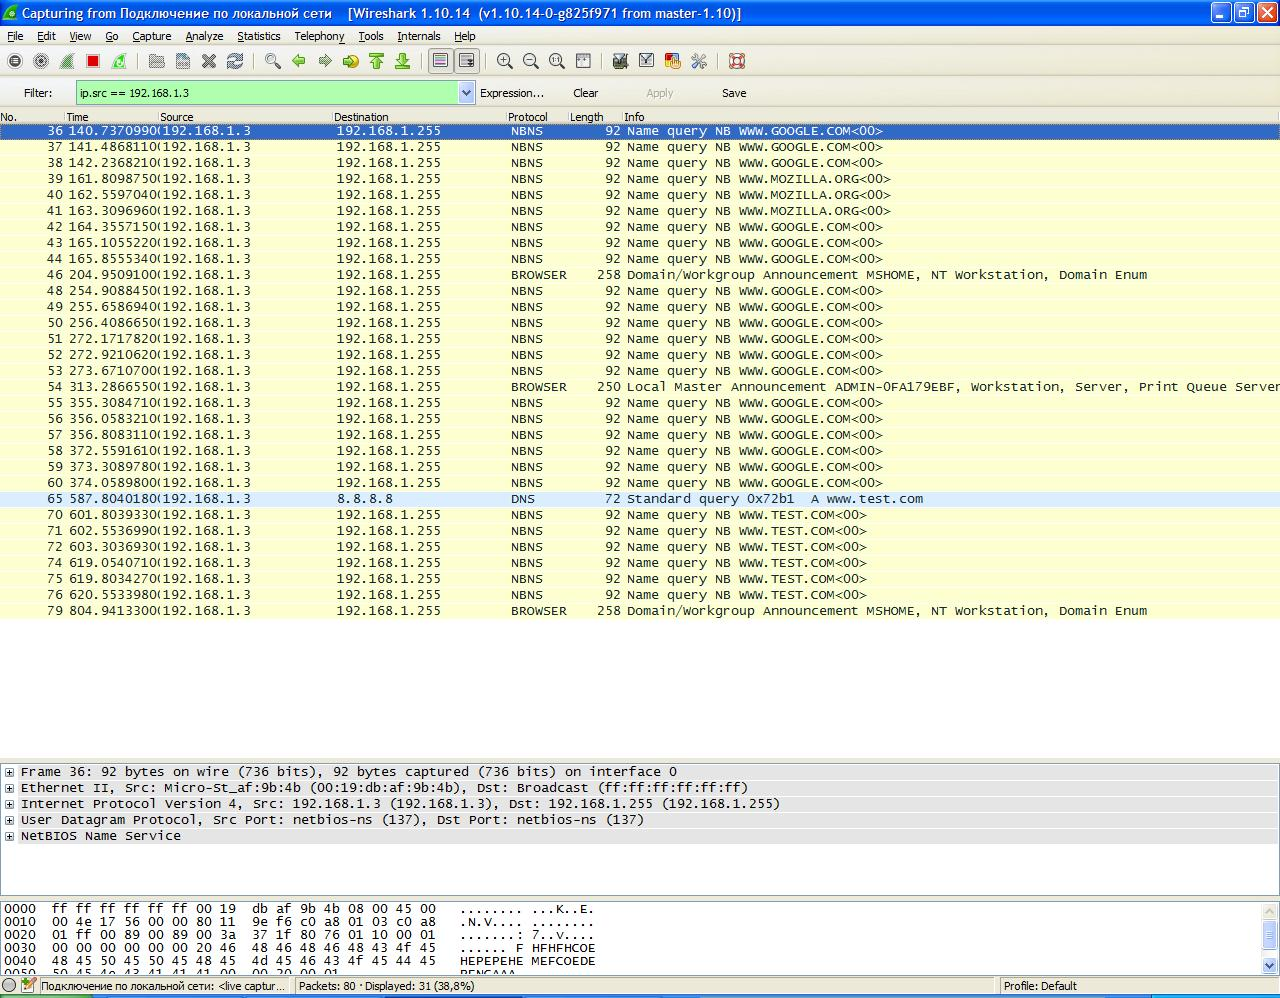
\includegraphics[width=0.79\linewidth]{2.png}
\caption{Окно с вращающимися планетами}
\label{fig:mpr}
\end{figure}

%Изображение Меркурия
\begin{figure}[h]
\centering
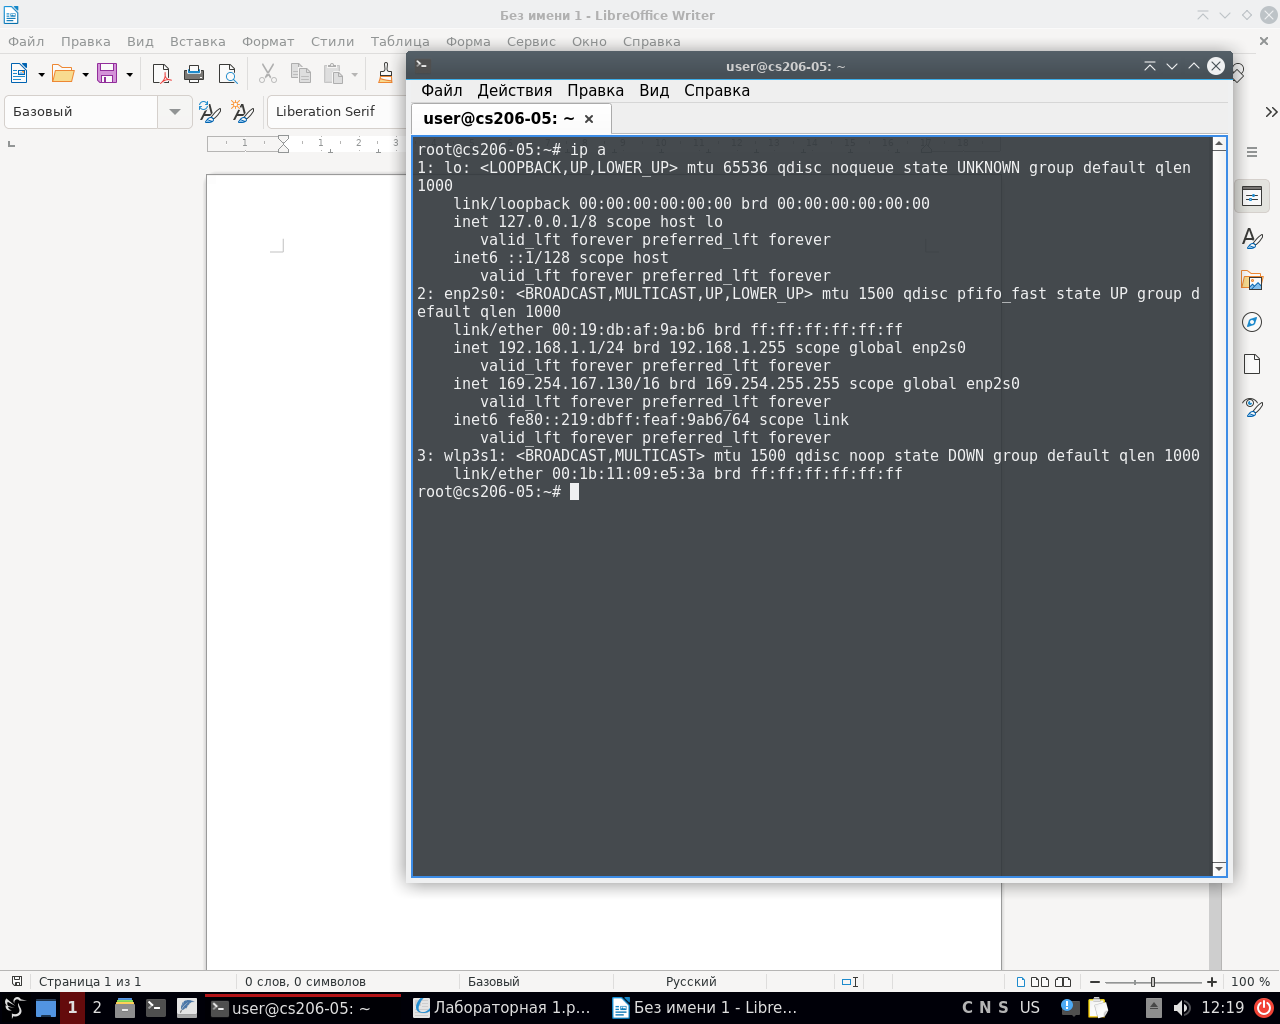
\includegraphics[width=0.78\linewidth]{1.png}
\caption{Итоговый вид окна info about planet}
\label{fig:mpr}

\end{figure}
%Изображение Меркурия
\begin{figure}[h]
\centering
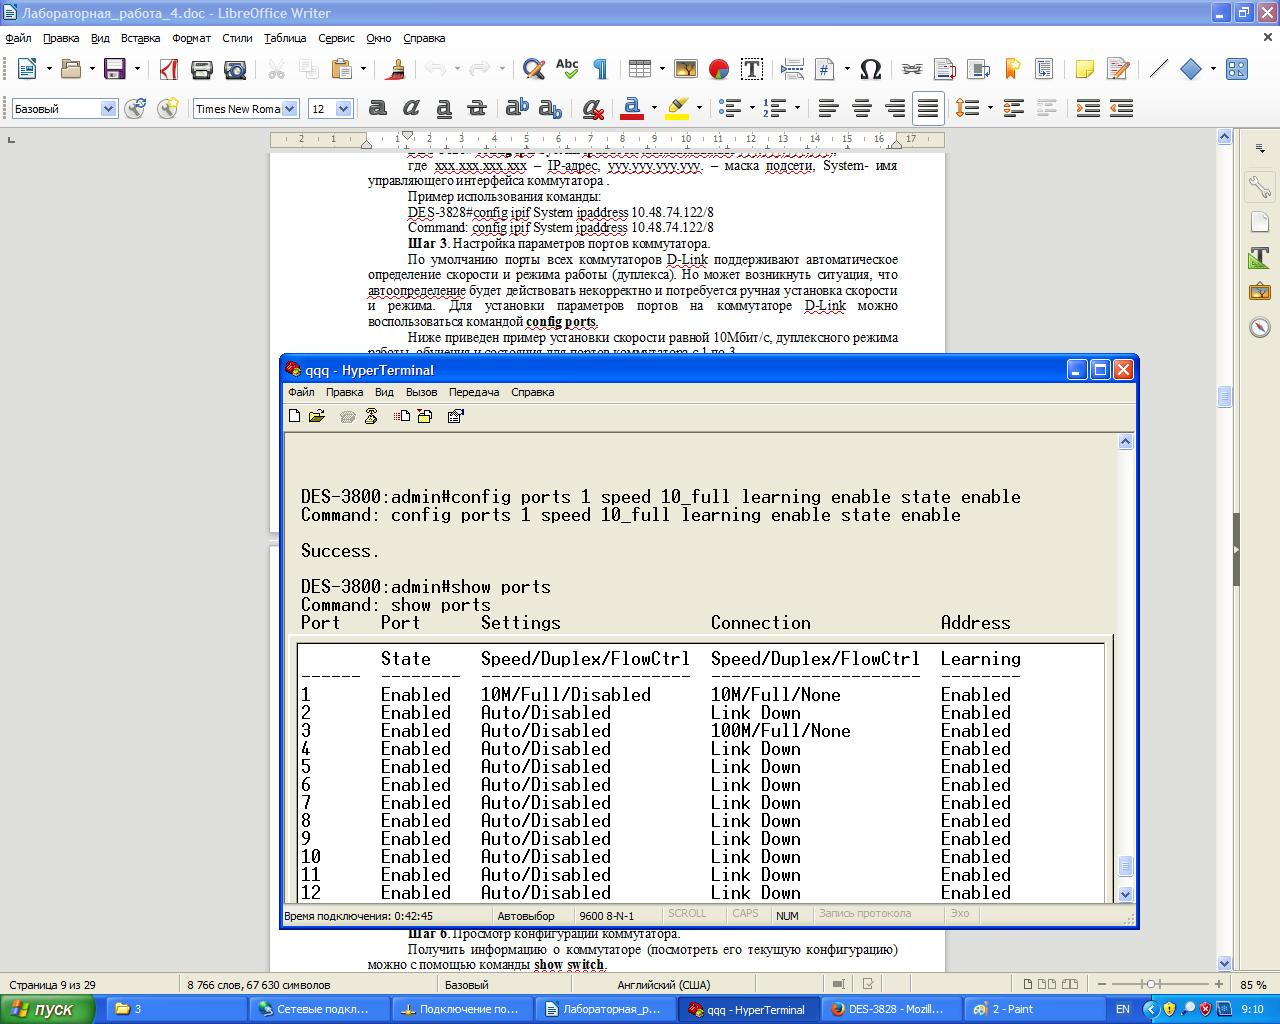
\includegraphics[width=1.0\linewidth]{3.png}
\caption{Диаграмма зависимости классов Planet и UI}
\label{fig:mpr}
\end{figure}



\begin{thebibliography}{5}
\bibitem{1}
https://www.python.org/
\bibitem{2}
https://younglinux.info/tkinter/menu.php
\bibitem{3}
https://ru.wikiversity.org/wiki/Tkinter
\bibitem{4}
https://v-kosmose.com/planetyi-solnechnoy-sistemyi/
\bibitem{5}
https://webfanat.com/article\_id/?id=117
\bibitem{6}
https://ru.wikipedia.org/wiki/Tkinter
\bibitem{7}
https://ru.wikipedia.org/wiki/Pythonhttps://ru.wikipedia.org/wiki/Python
\end{thebibliography}
\end{document}